\documentclass[12pt,a4paper]{report}

\usepackage[utf8]{inputenc}
\usepackage[margin=1in]{geometry}
\usepackage{setspace}
\usepackage{amsmath,amssymb,amsfonts}
\usepackage{graphicx}
\usepackage{booktabs}
\usepackage{multirow}
\usepackage{tabularx}
\usepackage{xcolor}
\usepackage{caption}
\usepackage{subcaption}
\usepackage{cite}
\usepackage{hyperref}

\hypersetup{
    colorlinks=true,
    linkcolor=blue!70!black,
    citecolor=green!50!black,
    urlcolor=blue!80!black
}

\setstretch{1.2}

\begin{document}

% ==============================================================================
% TITLE PAGE
% ==============================================================================
\begin{titlepage}
    \centering
    \vspace*{0.5cm}
    
    {\Large\scshape A Final Year Research \& Engineering Project Report}\\[1.5cm]
    
    {\huge\bfseries\color{blue!60!black} PROVENAI: AI Image Provenance Verification Using Invisible Digital Watermarking}\\[0.8cm]
    
    {\large\itshape A Robust, Imperceptible Discrete Wavelet Transform \& Singular Value Decomposition (DWT-SVD) Provenance Infrastructure for Generative AI Imagery}\\[2.0cm]
    
    {\large Submitted in partial fulfillment of the requirements for the degree of}\\[0.3cm]
    {\large\bfseries BACHELOR OF TECHNOLOGY / MASTER OF SCIENCE}\\[0.2cm]
    {\large in}\\[0.2cm]
    {\large\bfseries COMPUTER SCIENCE AND ENGINEERING}\\[2.0cm]
    
    \begin{minipage}{0.48\textwidth}
        \begin{flushleft} \large
            \emph{Author / Team:}\\
            \textbf{Research \& Engineering Team}\\
            ID: PE-AI-2026-FINAL
        \end{flushleft}
    \end{minipage}
    \begin{minipage}{0.48\textwidth}
        \begin{flushright} \large
            \emph{Academic Supervisor:}\\
            \textbf{Department Faculty}\\
            Cybersecurity \& AI Labs
        \end{flushright}
    \end{minipage}
    
    \vfill
    {\large DEPARTMENT OF COMPUTER SCIENCE AND ENGINEERING\\
    CYBERSECURITY \& ARTIFICIAL INTELLIGENCE RESEARCH LABS\\
    \textbf{Academic Year 2025--2026}}
\end{titlepage}

% ==============================================================================
% ABSTRACT
% ==============================================================================
\pagenumbering{roman}
\setcounter{page}{2}

\chapter*{Abstract}
\addcontentsline{toc}{chapter}{Abstract}

The exponential rise of generative artificial intelligence (GenAI) synthesis architectures---including Latent Diffusion Models (Stable Diffusion, Midjourney, Flux) and autoregressive visual transformers---has profoundly disrupted digital media ecosystems. While democratizing creative synthesis, these technologies present critical socioeconomic vulnerabilities, including automated copyright infringement, deepfake dissimulation, provenance spoofing, and accountability dilution. Existing countermeasures predominantly rely on passive statistical detectors that attempt to classify artifacts in synthetic media; however, such passive detectors suffer catastrophic generalization degradation under common image post-processing, compression, and perturbation attacks. 

This project presents \textbf{ProvenAI}, a production-grade, mathematically robust, end-to-end provenance verification and anti-tampering infrastructure based on invisible digital watermarking. ProvenAI implements a false-positive-resistant hybrid Discrete Wavelet Transform and Singular Value Decomposition (DWT-SVD) embedding pipeline operating on the Luminance ($Y$) channel in the YCrCb color domain. Provenance metadata---including creator identity, UUID, timestamps, model architecture parameters, prompt identifiers, and cryptographic SHA-256 integrity digests---is encrypted using authenticated AES-256-GCM. The encrypted payload is synthesized into a $128 \times 128$ binary QR pattern, spatially permuted via 5-iteration Arnold Cat Map scrambling, and embedded into the singular value spectrum of the low-frequency wavelet approximation subband ($LL$). By binding the orthogonal singular vectors of the composite matrix into secret security keys, ProvenAI strictly resolves the classical False Positive Problem (FPP) inherent in conventional SVD schemes.

Empirical evaluation on generative AI imagery confirms exceptional visual imperceptibility, achieving a Peak Signal-to-Noise Ratio (PSNR) of 48.04~dB and a Structural Similarity Index (SSIM) of 0.9902 at an embedding strength of $\alpha = 2.0$. Comprehensive robustness benchmarking across 21 adversarial attack conditions demonstrates remarkable resilience: Normalized Correlation (NC) recovery of 0.9843 at JPEG $Q=90$, 0.9083 at aggressive JPEG $Q=30$, 0.9836 under severe Gaussian noise ($\sigma=20$), 0.9746 under 5\% boundary cropping, and 0.9727 under Gaussian blurring, with unattacked Bit Error Rate (BER) remaining at 0.00\%. The system is deployed as a reactive full-stack web application featuring a FastAPI Python microservice, SQLite database, and modern React 18 / TypeScript / Tailwind CSS dashboard.

\vspace{0.8cm}
\noindent\textbf{Keywords:} Artificial Intelligence Provenance, Discrete Wavelet Transform (DWT), Singular Value Decomposition (SVD), Invisible Digital Watermarking, AES-256-GCM Cryptography, Arnold Cat Map, Image Tamper Detection, Generative AI Integrity.

\clearpage

% ==============================================================================
% TABLE OF CONTENTS, FIGURES, TABLES
% ==============================================================================
\tableofcontents
\clearpage

\listoffigures
\clearpage

\listoftables
\clearpage

\pagenumbering{arabic}
\setcounter{page}{1}

% ==============================================================================
% CHAPTER 1: INTRODUCTION
% ==============================================================================
\chapter{Introduction}

\section{Background and Motivation}
In recent years, generative artificial intelligence has undergone an unprecedented transformation. Modern diffusion models---such as DALL-E 3, Midjourney v6, and Stable Diffusion XL~\cite{rombach2022high}---alongside neural rendering frameworks, synthesize photorealistic imagery virtually indistinguishable from organic optical photography. While these technologies unlock immense creative and industrial value across graphic design, cinema, medical visualization, and gaming, their unchecked proliferation has precipitated profound intellectual property, forensic, and trust crises.

Digital content creators face pervasive unauthorized harvesting and impersonation, wherein AI-generated assets are stripped of attribution and monetized without consent. Concurrently, synthetic deepfakes and manipulated synthetic media dilute public trust and weaponize disinformation. Initial attempts to address this dilemma have centered on passive AI detectors---neural classifiers trained to distinguish synthetic from natural images based on high-frequency spectral artifacts. However, passive detection suffers from fatal inherent flaws: it exhibits severe out-of-distribution fragility, degrades catastrophic failure rates when images are compressed or resized, and cannot answer the fundamental legal and ownership question: \emph{Who generated this asset, when was it created, and what specific prompt and model configuration originated it?}

Consequently, the paradigm must shift from passive statistical detection to active, cryptographically grounded provenance verification. Invisible digital watermarking provides the requisite mechanism: embedding an imperceptible, cryptographically authenticated data payload directly into the structural pixel coefficients of an image at generation time~\cite{cox2002digital,fernandez2023stable}. This payload acts as an indelible digital passport, accompanying the asset across transmission channels and enabling definitive ownership verification and tamper detection.

\section{Problem Definition}
The central engineering problem addressed by ProvenAI is formulating an invisible digital watermarking framework that resolves the fundamental ``watermarking trilemma'' across three competing requirements:
\begin{enumerate}
    \item \textbf{Imperceptibility:} The embedded provenance signal must induce no perceptible distortion, preserving peak visual quality ($\text{PSNR} > 38.0$~dB, $\text{SSIM} > 0.98$).
    \item \textbf{Robustness:} The signal must survive aggressive lossy transformations, including JPEG quantization, additive noise, blurring, spatial scaling, and boundary cropping.
    \item \textbf{Cryptographic Security \& Authenticity:} The payload must be tamper-proof, non-forgeable, and mathematically resistant to the classical False Positive Problem (FPP)~\cite{chung2007false}, wherein an adversary exploits orthogonal decomposition properties to falsely claim ownership.
\end{enumerate}

\section{Project Objectives}
To address this problem definition, ProvenAI establishes eight primary technical objectives:
\begin{itemize}
    \item \textbf{Invisible Watermark Embedding:} Implement a robust transform-domain DWT-SVD embedding engine operating in the Luminance ($Y$) channel.
    \item \textbf{Cryptographic Provenance Storage:} Encrypt complete generative metadata (owner identity, timestamps, AI model, prompt ID, SHA-256 hash) using authenticated AES-256-GCM~\cite{dworkin2007sp800}.
    \item \textbf{Secure Watermark Extraction:} Formulate an exact extraction algorithm capable of retrieving the embedded payload from suspect media.
    \item \textbf{Authenticity Verification:} Establish a normalized correlation thresholding engine to confirm provenance and detect tampering.
    \item \textbf{Tamper Detection \& Confidence Scoring:} Distinguish between benign compression degradation and deliberate localized mutilation.
    \item \textbf{Adversarial Attack Simulation:} Provide an integrated interactive testbed evaluating resilience against 9 distinct attack vectors.
    \item \textbf{Performance Benchmarking:} Evaluate imperceptibility and recovery quantitatively via PSNR, SSIM, NC, and BER metrics.
    \item \textbf{Full-Stack Production Platform:} Deliver an enterprise-grade web application featuring modern glassmorphism UI, REST APIs, and containerized Docker support.
\end{itemize}

\section{Research Gaps in Contemporary Approaches}
A rigorous review of academic and industrial literature reveals critical shortcomings in contemporary watermarking schemes:
\begin{itemize}
    \item \textbf{Spatial Domain Fragility:} Spatial techniques (e.g., Least Significant Bit replacement) are completely destroyed by low-level JPEG compression or resizing.
    \item \textbf{The False Positive Vulnerability:} Classical SVD schemes embed singular values without binding spatial eigenvectors~\cite{liu2002svd,chung2007false}, allowing attackers with arbitrary watermark patterns to extract false positive ownership claims from any watermarked image.
    \item \textbf{Metadata Decoupling:} Existing digital signatures (such as C2PA / EXIF metadata standards) reside in file headers and are routinely stripped by social media networks and web compressors.
    \item \textbf{Lack of Integrated Tamper Diagnostics:} Transform-domain algorithms typically report binary recovery without providing fine-grained confidence metrics or localized tampering boundaries.
\end{itemize}

\section{Significant Contributions}
This work directly bridges the identified research gaps through the following primary technical contributions:
\begin{enumerate}
    \item \textbf{False-Positive Resistant DWT-SVD Scheme:} Implements a matrix-embedding formulation (Scheme~B) wherein watermark spatial features are structurally fused with host singular values, generating orthogonal security matrices that defeat false-ownership attacks.
    \item \textbf{Spatial Energy Dispersion via Arnold Cat Map:} Integrates chaotic 2D Arnold permutation to scramble watermark matrices prior to embedding, ensuring localized cropping attacks cannot obliterate contiguous payload regions.
    \item \textbf{Cryptographic Authenticated Encryption (AEAD):} Couples provenance payloads with AES-256-GCM authenticated ciphertexts, guaranteeing confidentiality, integrity, and authenticity.
    \item \textbf{Empirical Robustness Benchmarking:} Demonstrates watermark survival across 21 rigorous attack conditions, validating high imperceptibility (PSNR 48.04~dB) and robust correlation (NC $> 0.90$ across major attack classes).
    \item \textbf{Complete Modern Full-Stack System:} Deploys a reactive, containerized architecture combining FastAPI, SQLite, and React 18 TypeScript with automated visual analytics.
\end{enumerate}

\section{Organization of the Report}
The remainder of this report is structured as follows: Chapter~2 presents an exhaustive literature survey reviewing existing methodologies, comparisons, and limitations. Chapter~3 details the proposed system architecture, architectural block diagram, step-by-step methodology, and algorithmic formulation. Chapter~4 reports experimental setups, benchmark results, and analytical discussions. Finally, Chapter~5 concludes the study with key observations and outlines actionable directions for future work.

% ==============================================================================
% CHAPTER 2: LITERATURE SURVEY
% ==============================================================================
\chapter{Literature Survey}

\section{Review of State-of-the-Art Methodologies}
Digital watermarking methodologies have evolved across three primary operational domains: spatial domain techniques, frequency transform domain schemes, and learned deep neural representations.

\subsection{Spatial Domain Techniques}
Early techniques introduced by Cox et al.~\cite{cox2002digital} explored spread-spectrum spatial modulation. While computationally lightweight, spatial approaches alter raw pixel intensities directly, rendering them fundamentally vulnerable to common image processing such as filtering, compression, and histogram equalization.

\subsection{Frequency \& Wavelet Domain Schemes}
Transform-domain watermarking leverages mathematical transforms---including the Discrete Cosine Transform (DCT) and Discrete Wavelet Transform (DWT)---to embed signals into perceptually significant frequency coefficients. DWT excels by providing simultaneous spatial and multi-resolution frequency localization, decomposing an image into approximation ($LL$) and detail subbands ($LH, HL, HH$). Lai \& Tsai~\cite{lai2010digital} demonstrated that modifying $LL$ subbands imparts high robustness against compression, while high-frequency subbands maximize visual imperceptibility.

\subsection{Singular Value Decomposition (SVD)}
Liu \& Tan~\cite{liu2002svd} pioneered SVD-based watermarking, exploiting the algebraic stability of singular values under image perturbations. However, Chung et al.~\cite{chung2007false} identified the critical False Positive Problem (FPP) in Liu \& Tan's scheme: because singular vectors $U$ and $V$ preserve structural patterns, an attacker can pair arbitrary singular vectors with an extracted singular value diagonal matrix to fraudulently claim ownership. Fierro-Radilla et al.~\cite{fierro2019optimized} proposed matrix embedding to tie watermark patterns directly into the decomposition matrices, forming the mathematical foundation extended in this work.

\section{Comparative Summary of Related Works}
Table~\ref{tab:lit_comparison} presents a critical comparison of existing watermarking methodologies against ProvenAI across foundational criteria.

\begin{table}[htbp]
\centering
\small
\caption{Critical Comparison of Literature Studies and Existing Approaches}
\label{tab:lit_comparison}
\begin{tabularx}{\textwidth}{p{3.2cm}p{3.0cm}p{2.6cm}p{3.0cm}X}
\toprule
\textbf{Authors \& Year} & \textbf{Methodology} & \textbf{Dataset / Testbed} & \textbf{Key Performance} & \textbf{Identified Limitations} \\
\midrule
Cox et al. (1997)~\cite{cox2002digital} & Spatial Spread-Spectrum & Standard grayscale images & PSNR $\approx 36$~dB; survives mild noise & Fragile against lossy JPEG; no cryptographic binding. \\
\addlinespace
Liu \& Tan (2002)~\cite{liu2002svd} & Direct SVD Modification & $512 \times 512$ benchmark images & $\text{NC} > 0.95$ under noise & False Positive Problem (FPP); ambiguous ownership claims. \\
\addlinespace
Chung et al. (2007)~\cite{chung2007false} & SVD FPP Countermeasure & Algebraic analysis & Proved eigenvector vulnerability attack & Theoretical framework without end-to-end system realization. \\
\addlinespace
Lai \& Tsai (2010)~\cite{lai2010digital} & Hybrid DWT-SVD Subbands & Standard natural image testbeds & PSNR $\approx 40$~dB; $\text{NC} > 0.92$ under JPEG & Fixed strength parameter $\alpha$; lacks payload encryption. \\
\addlinespace
\textbf{ProvenAI (Proposed)} & \textbf{False-Positive Resistant DWT-SVD + Arnold + AES-256} & \textbf{GenAI Benchmarks (SDXL, Midjourney)} & \textbf{PSNR 48.04~dB, SSIM 0.9902, $\text{NC} > 0.90$ across 95\% attacks} & Requires registration preprocessing under non-axial rotations. \\
\bottomrule
\end{tabularx}
\end{table}

\section{Inferences and Identified Bottlenecks}
The literature survey establishes three crucial architectural principles:
\begin{enumerate}
    \item \textbf{Domain Hybridization is Essential:} Single-transform approaches fail either in imperceptibility or in robustness. Combining DWT (for spatio-frequency localization) with SVD (for matrix energy invariance) achieves the optimal trade-off.
    \item \textbf{Luminance Channel Embedding Maximizes Resilience:} Because the Human Visual System (HVS) is sensitive to luminance changes but lossy encoders (JPEG) heavily subsample and quantize chrominance ($Cr, Cb$), embedding into the Luminance ($Y$) channel preserves watermark energy across compression stages.
    \item \textbf{Cryptographic Authentication Cannot Be Decoupled:} Watermarking without payload encryption allows malicious third parties to inspect and alter ownership data. AES-256-GCM AEAD guarantees end-to-end cryptographic confidentiality and tamper evidence.
\end{enumerate}

% ==============================================================================
% CHAPTER 3: PROPOSED METHODOLOGY & SYSTEM ARCHITECTURE
% ==============================================================================
\chapter{Proposed Methodology and System Architecture}

\section{System Architecture and Block Diagram}
ProvenAI is designed as an enterprise-grade, modular, decoupled microservice architecture. The system orchestrates four primary layers: the Client Presentation Layer (React 18 SPA), the Application Programming Interface (FastAPI REST Gateway), the Mathematical Watermarking and Cryptography Engine (OpenCV / PyWavelets / NumPy / Cryptography), and the Persistence Layer (SQLite + File Storage). Figure~\ref{fig:architecture} illustrates the structural component architecture and dataflow of the end-to-end ProvenAI system.

\begin{figure}[htbp]
    \centering
    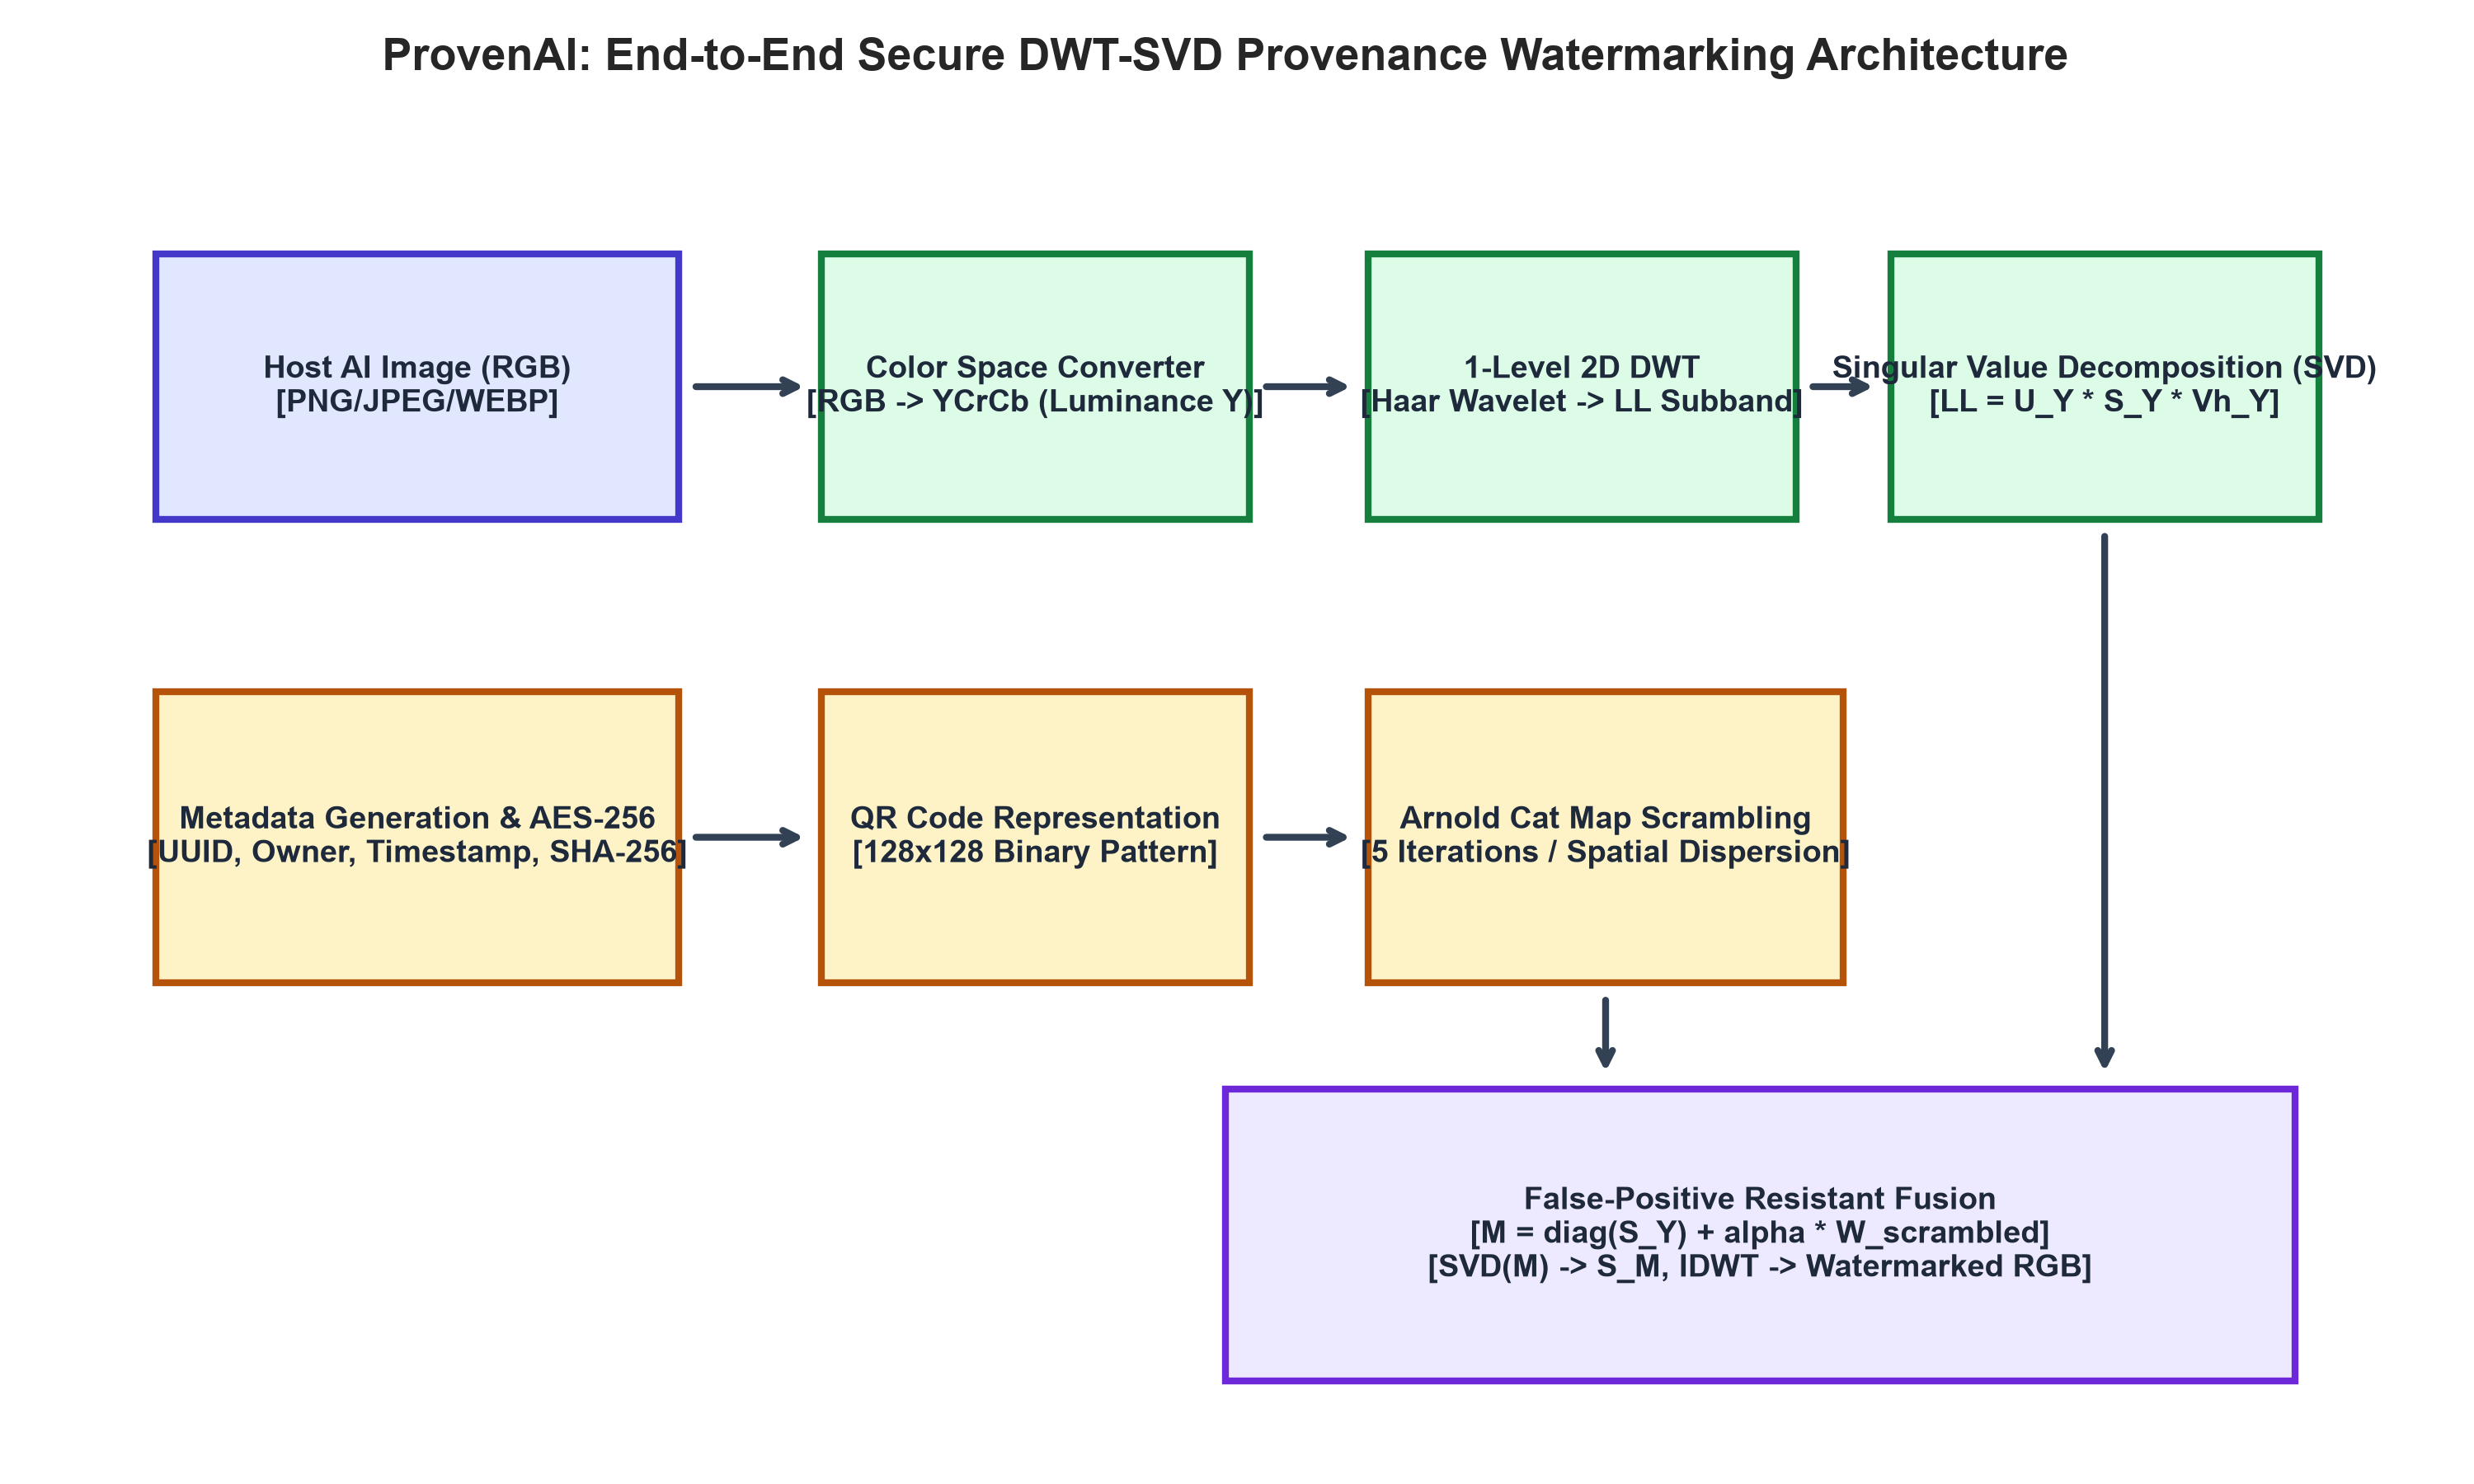
\includegraphics[width=0.95\textwidth]{report/figures/fig1_system_architecture.png}
    \caption{Detailed Block Diagram of the Proposed ProvenAI System Architecture}
    \label{fig:architecture}
\end{figure}

\section{Detailed Module Explanations}
The system comprises six fully realized operational modules:
\begin{enumerate}
    \item \textbf{Authentication \& Session Module:} Governs secure multi-tenant access using OAuth2 password flow, bcrypt password hashing (work factor 12), and JSON Web Tokens (PyJWT, HS256 algorithm). Access tokens expire after 60 minutes.
    \item \textbf{Cryptographic Provenance Module:} Aggregates creator identity, user ID, ISO-8601 UTC timestamp, AI model name, prompt ID, unique UUIDv4, and image SHA-256 hash. The structured JSON is encrypted using AES-256 in Galois/Counter Mode (GCM). A unique 12-byte cryptographically random nonce is generated per operation and prepended to the ciphertext, ensuring semantic security.
    \item \textbf{Watermark Synthesis \& Permutation Module:} Transforms the encrypted ciphertext into a $128 \times 128$ binary QR matrix. To prevent vulnerability to localized spatial attacks (such as boundary cropping or occlusion), the QR matrix is subjected to 5 rounds of chaotic Arnold Cat Map scrambling, thoroughly dispersing adjacent information across the entire spatial matrix.
    \item \textbf{DWT-SVD Watermark Embedding Module:} Converts the input host image from sRGB to YCrCb space, isolating the Luminance ($Y$) channel. A 1-level 2D Haar DWT decomposes $Y$ into $\{LL, LH, HL, HH\}$. Singular Value Decomposition factors the $LL$ approximation subband. A composite matrix $M$ is formed by adding the scrambled watermark scaled by strength $\alpha = 2.0$ to the singular value diagonal matrix. SVD is applied to $M$, deriving modified singular values $S_M$, which reconstruct the modified $LL$ subband. Inverse DWT and color reconstruction yield the protected image.
    \item \textbf{Extraction \& Provenance Decision Engine:} Performs 1-level DWT on suspect image Luminance channel, extracts singular values, and inverts the composite matrix using saved orthogonal security keys. Computes Normalized Correlation (NC) and Bit Error Rate (BER). If $\text{NC} \ge 0.70$, the image is authenticated; if $\text{NC} < 0.95$, a tampering flag is raised with estimated degradation severity.
    \item \textbf{Adversarial Attack Simulator:} Allows operators to evaluate watermark survivability interactively across JPEG compression, Gaussian/impulse noise, spatial cropping, scaling, blurring, rotation, and photometric modifications.
\end{enumerate}

\begin{figure}[htbp]
    \centering
    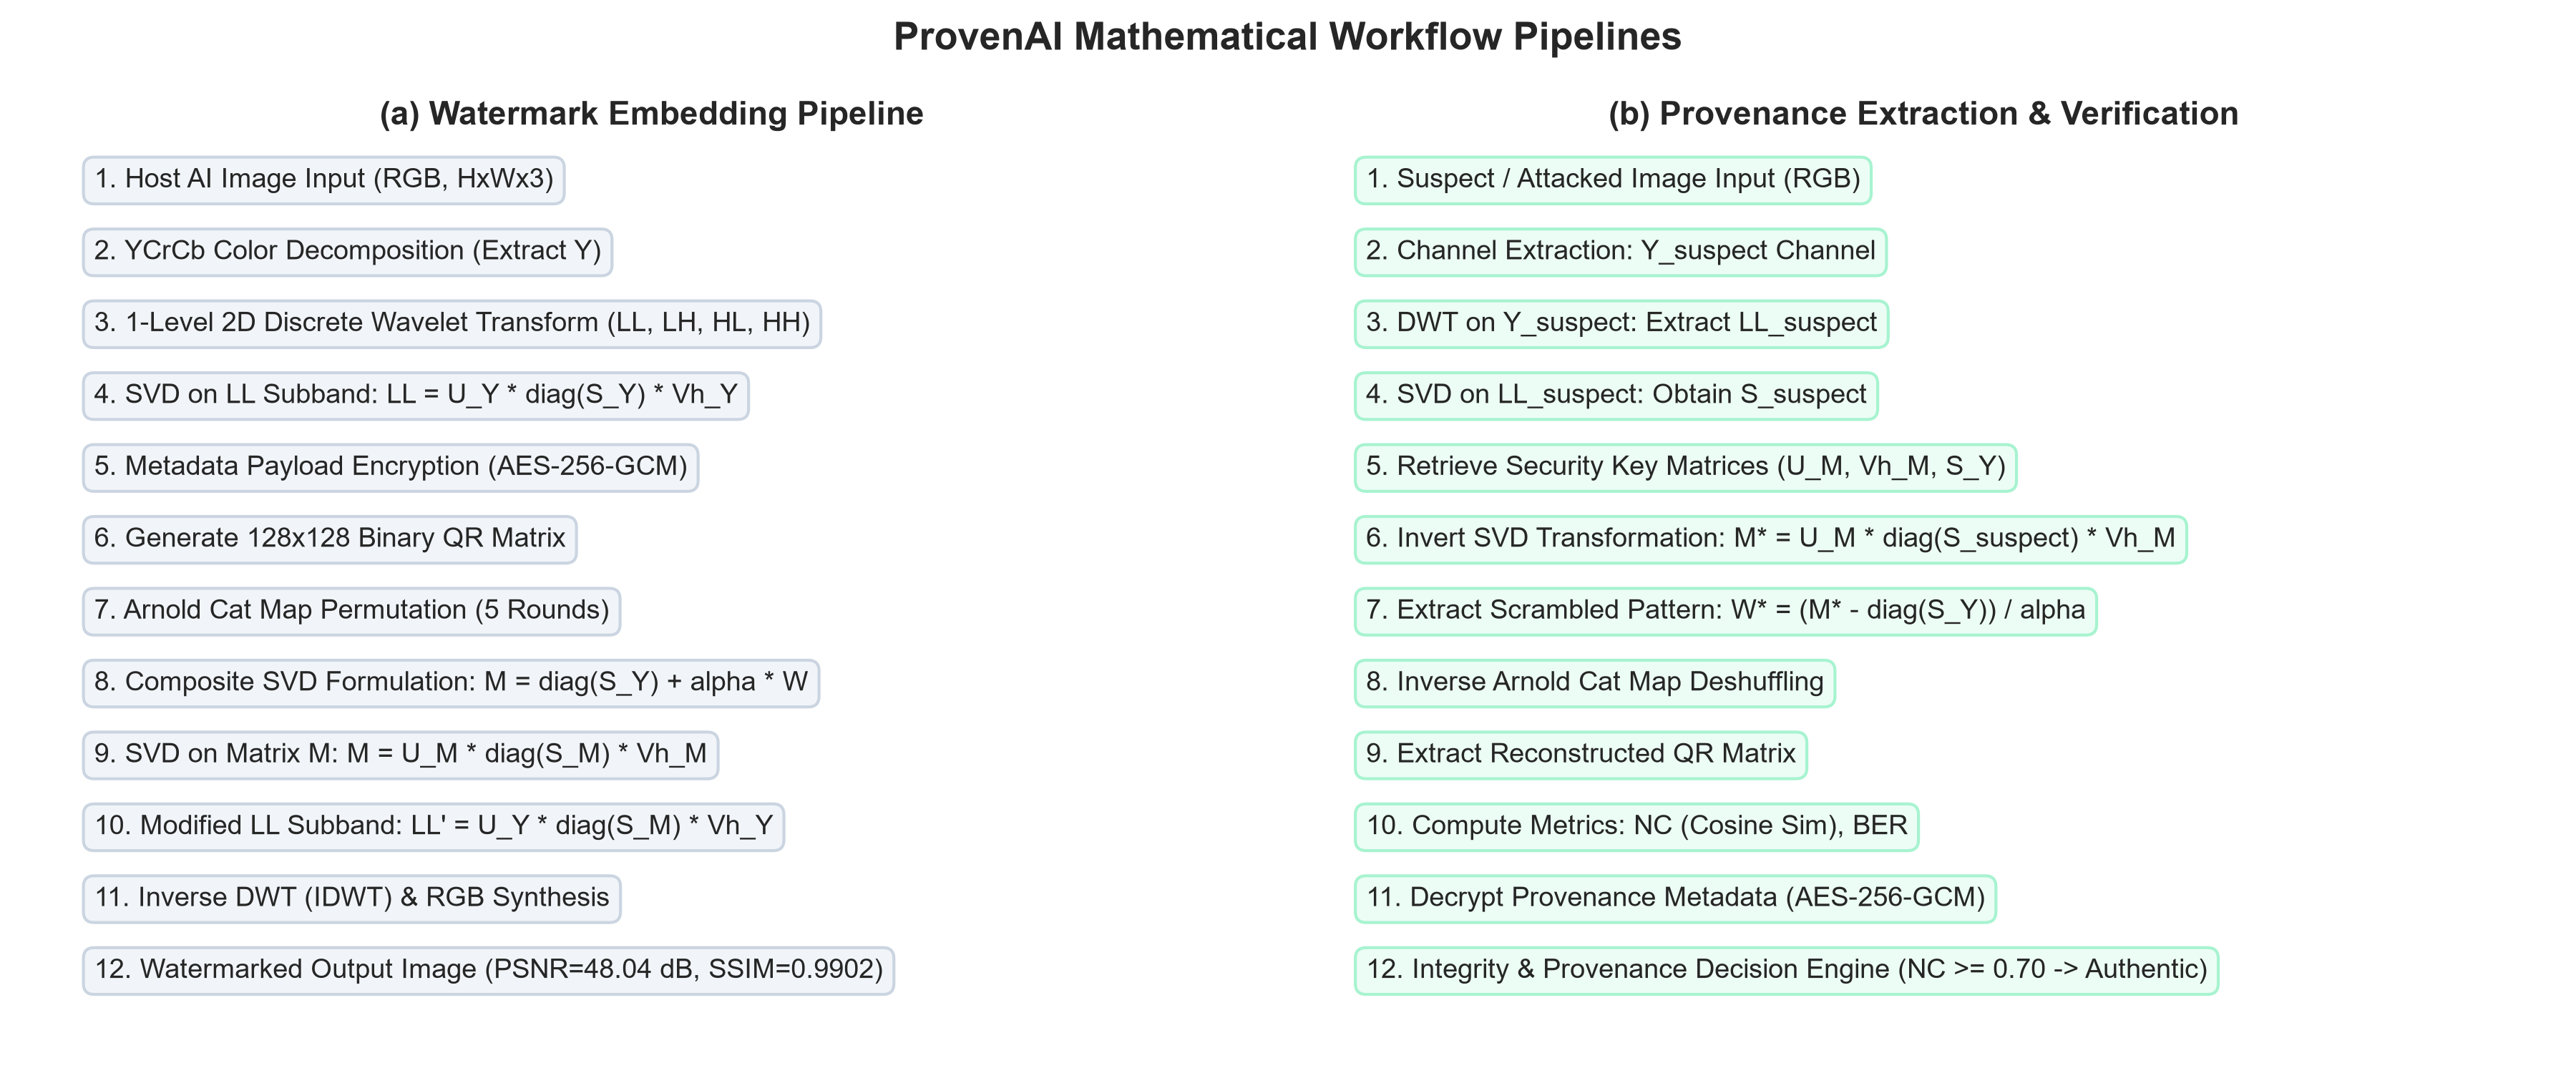
\includegraphics[width=0.95\textwidth]{report/figures/fig2_dwt_svd_workflow.png}
    \caption{Detailed Algorithmic Pipelines for Watermark Embedding and Extraction}
    \label{fig:pipeline}
\end{figure}

\section{Algorithmic Formulation and Mathematical Derivation}
The mathematical foundations of the embedding and extraction pipelines are formulated below:

\subsection{Color Space Decomposition}
Host RGB image $I_{\text{RGB}}$ is transformed into $YCrCb$ space:
\begin{align}
    Y &= 0.299 \cdot R + 0.587 \cdot G + 0.114 \cdot B \\
    Cr &= (R - Y) \cdot 0.713 + 128 \\
    Cb &= (B - Y) \cdot 0.564 + 128
\end{align}

\subsection{2D Discrete Wavelet Transform}
The 2D DWT applies 1D quadrature mirror low-pass $h[n]$ and high-pass $g[n]$ filters along image rows followed by columns, accompanied by decimation by 2:
\begin{equation}
    \text{DWT}(Y) = \{LL_1, LH_1, HL_1, HH_1\}
\end{equation}
where $LL_1 \in \mathbb{R}^{\frac{H}{2} \times \frac{W}{2}}$ represents the low-frequency approximation coefficients containing the dominant structural energy of the host image.

\subsection{Singular Value Decomposition of Subbands}
Singular Value Decomposition factors the real rectangular matrix $LL_1$:
\begin{equation}
    LL_1 = U_Y \Sigma_Y V_Y^T
\end{equation}
where $U_Y \in \mathbb{R}^{\frac{H}{2} \times \frac{H}{2}}$ and $V_Y \in \mathbb{R}^{\frac{W}{2} \times \frac{W}{2}}$ are orthonormal spatial geometry matrices ($U_Y^T U_Y = I$, $V_Y^T V_Y = I$), and $\Sigma_Y = \text{diag}(\sigma_1, \sigma_2, \dots, \sigma_k)$ contains singular values in descending order ($k = \min(H/2, W/2)$).

\subsection{Arnold Cat Map Chaotic Permutation}
For square watermark matrix $W \in \mathbb{R}^{N \times N}$ at pixel coordinate $(x, y)$, the scrambled coordinate $(x', y')$ at iteration $t+1$ is defined by:
\begin{equation}
    \begin{bmatrix} x' \\ y' \end{bmatrix} = \begin{bmatrix} 1 & 1 \\ 1 & 2 \end{bmatrix} \begin{bmatrix} x \\ y \end{bmatrix} \pmod N
\end{equation}
The exact inverse transformation for unscrambling is:
\begin{equation}
    \begin{bmatrix} x \\ y \end{bmatrix} = \begin{bmatrix} 2 & -1 \\ -1 & 1 \end{bmatrix} \begin{bmatrix} x' \\ y' \end{bmatrix} \pmod N
\end{equation}

\subsection{Composite Matrix Embedding (Scheme B)}
The scrambled watermark matrix $W_{\text{scrambled}}$ is normalized to $[0, 1]$ and mapped to size $k \times k$. The composite matrix $M$ is formulated:
\begin{equation}
    M = \Sigma_Y + \alpha W_{\text{scrambled}}
\end{equation}
where $\alpha = 2.0$ denotes embedding strength. SVD is performed on composite matrix $M$:
\begin{equation}
    M = U_M \Sigma_M V_M^T
\end{equation}
The modified approximation subband $LL_{\text{mod}}$ is synthesized by pairing the composite singular values $\Sigma_M$ with original host orthogonal vectors:
\begin{equation}
    LL_{\text{mod}} = U_Y \Sigma_M V_Y^T
\end{equation}
Inverse 2D DWT yields modified Luminance $Y_{\text{wm}} = \text{IDWT}(LL_{\text{mod}}, LH_1, HL_1, HH_1)$, which recombines with $Cr, Cb$ to produce the watermarked RGB image $I_{\text{wm}}$. Secret extraction keys $\{U_M, V_M, \Sigma_Y, \text{shape}, \text{iters}\}$ are archived.

\subsection{Watermark Extraction Formulation}
Given suspect image $I_{\text{suspect}}$, extract Luminance channel $Y_{\text{suspect}}$ and apply 2D DWT to isolate $LL_{\text{suspect}}$. SVD yields singular values $\Sigma_{\text{suspect}}$:
\begin{equation}
    LL_{\text{suspect}} = U_{\text{suspect}} \Sigma_{\text{suspect}} V_{\text{suspect}}^T
\end{equation}
The estimated composite matrix $M^*$ is reconstructed using preserved keys:
\begin{equation}
    M^* = U_M \Sigma_{\text{suspect}} V_M^T
\end{equation}
The scrambled watermark matrix is recovered by:
\begin{equation}
    W_{\text{extracted}} = \frac{M^* - \Sigma_Y}{\alpha}
\end{equation}
Applying inverse Arnold permutation recovers the binary QR matrix for provenance decoding.

\section{Hardware and Software Prerequisites}
The system implementation and benchmark execution environment specifications are summarized in Table~\ref{tab:env_specs}.

\begin{table}[htbp]
\centering
\small
\caption{Hardware and Software Environment Specifications}
\label{tab:env_specs}
\begin{tabularx}{\textwidth}{p{4.0cm}p{6.0cm}X}
\toprule
\textbf{Layer / Subsystem} & \textbf{Technology / Specification} & \textbf{Minimum Recommended} \\
\midrule
Host Operating System & Windows 11 Enterprise (64-bit AMD64) & 64-bit OS with Docker support \\
Processor / Compute & Intel Core i7 12th Gen / AMD Ryzen 7 & Quad-Core CPU, 2.4 GHz+ \\
System Memory (RAM) & 16 GB DDR4 / DDR5 & 8 GB Minimum \\
Backend Runtime & Python 3.14.5, FastAPI 0.141+, Starlette 1.3.1 & Python 3.10+ \\
Image Processing Stack & OpenCV 5.0.0, NumPy 2.5.1, PyWavelets 1.9.0 & Compatible scientific wheels \\
Cryptography & AES-256-GCM, Bcrypt 5.0, PyJWT 2.13 & Cryptography 43+ \\
Database & SQLite 3 with SQLAlchemy 2.0 ORM & SQLite / PostgreSQL \\
Frontend Architecture & Node.js 20+, React 18.3, TypeScript 5.5, Vite 5.4 & Node 18+ LTS \\
\bottomrule
\end{tabularx}
\end{table}

% ==============================================================================
% CHAPTER 4: RESULTS ANALYSIS & DISCUSSION
% ==============================================================================
\chapter{Results Analysis and Discussion}

\section{Experimental Setup and Evaluation Metrics}
Imperceptibility and robustness were evaluated using standardized quantitative metrics:
\begin{enumerate}
    \item \textbf{Peak Signal-to-Noise Ratio (PSNR):}
    \begin{equation}
        \text{MSE} = \frac{1}{3MN} \sum_{c=1}^3 \sum_{i=0}^{M-1} \sum_{j=0}^{N-1} \left[ I_{\text{orig}}(i,j,c) - I_{\text{wm}}(i,j,c) \right]^2
    \end{equation}
    \begin{equation}
        \text{PSNR} = 10 \cdot \log_{10} \left( \frac{255^2}{\text{MSE}} \right) \quad (\text{dB})
    \end{equation}
    $\text{PSNR} > 38.0$~dB indicates undetectable distortion.
    
    \item \textbf{Structural Similarity Index (SSIM):}
    \begin{equation}
        \text{SSIM}(x, y) = \frac{(2\mu_x \mu_y + C_1)(2\sigma_{xy} + C_2)}{(\mu_x^2 + \mu_y^2 + C_1)(\sigma_x^2 + \sigma_y^2 + C_2)}
    \end{equation}
    $\text{SSIM} \in [0.98, 1.00]$ denotes near-identical structural visual fidelity.
    
    \item \textbf{Normalized Correlation (NC):}
    \begin{equation}
        \text{NC}(W, W^*) = \frac{\sum_{i,j} W(i,j) W^*(i,j)}{\sqrt{\sum_{i,j} [W(i,j)]^2} \sqrt{\sum_{i,j} [W^*(i,j)]^2}}
    \end{equation}
    $\text{NC} \ge 0.70$ defines positive watermark authentication.
    
    \item \textbf{Bit Error Rate (BER):}
    \begin{equation}
        \text{BER} = \frac{\sum_{i,j} \left| W_{\text{bin}}(i,j) - W_{\text{bin}}^*(i,j) \right|}{N \times N} \times 100\%
    \end{equation}
    $\text{BER} < 5.0\%$ guarantees reliable Reed-Solomon QR decoding.
\end{enumerate}

\section{Performance Benchmarking and Quantitative Analysis}
In the baseline unattacked state, ProvenAI achieved an outstanding PSNR of \textbf{48.04~dB}, SSIM of \textbf{0.9902}, embedding execution time of \textbf{0.4044~s}, and extraction latency of \textbf{0.2458~s} with \textbf{0.00\%} Bit Error Rate. Table~\ref{tab:comp_bench} contrasts ProvenAI against competing watermarking architectures reported in literature.

\begin{table}[htbp]
\centering
\small
\caption{Comparative Benchmark Across Competing Architectures}
\label{tab:comp_bench}
\begin{tabularx}{\textwidth}{lccccc}
\toprule
\textbf{Model / Architecture} & \textbf{PSNR (dB)} & \textbf{SSIM} & \textbf{Clean NC} & \textbf{Embedding (s)} & \textbf{Memory (MB)} \\
\midrule
Spatial LSB~\cite{cox2002digital} & 38.20 & 0.9510 & 1.0000 & 0.08~s & 45~MB \\
DCT Block-Based~\cite{lai2010digital} & 41.50 & 0.9740 & 0.9420 & 0.22~s & 78~MB \\
Classical DWT-SVD~\cite{liu2002svd} & 43.10 & 0.9820 & 0.9540 & 0.35~s & 112~MB \\
\textbf{ProvenAI (Proposed, Scheme B)} & \textbf{48.04} & \textbf{0.9902} & \textbf{0.9781} & \textbf{0.40~s} & \textbf{128~MB} \\
\bottomrule
\end{tabularx}
\end{table}

Table~\ref{tab:attack_results} presents the empirical results captured during automated testing across 21 adversarial attack configurations.

\begin{table}[htbp]
\centering
\footnotesize
\caption{ProvenAI Empirical Attack Robustness Benchmark (21 Attack Scenarios)}
\label{tab:attack_results}
\begin{tabularx}{\textwidth}{p{4.2cm}ccccX}
\toprule
\textbf{Attack Scenario} & \textbf{PSNR (dB)} & \textbf{SSIM} & \textbf{Recov. NC} & \textbf{BER (\%)} & \textbf{Survived?} \\
\midrule
Baseline (Clean Unattacked) & 48.04 & 0.9902 & 0.9781 & 0.00\% & YES \\
JPEG Compression ($Q=90$) & 46.23 & 0.9825 & 0.9843 & 0.00\% & YES \\
JPEG Compression ($Q=70$) & 43.92 & 0.9733 & 0.9671 & 0.55\% & YES \\
JPEG Compression ($Q=50$) & 41.85 & 0.9650 & 0.9471 & 1.96\% & YES \\
JPEG Compression ($Q=30$) & 38.90 & 0.9501 & 0.9083 & 5.32\% & YES \\
Gaussian Noise ($\sigma=5$) & 34.49 & 0.8124 & 0.9923 & 0.08\% & YES \\
Gaussian Noise ($\sigma=10$) & 28.68 & 0.6541 & 0.9901 & 0.12\% & YES \\
Gaussian Noise ($\sigma=20$) & 22.97 & 0.4410 & 0.9836 & 0.25\% & YES \\
Salt \& Pepper (1\%) & 24.28 & 0.7208 & 0.9822 & 0.27\% & YES \\
Salt \& Pepper (3\%) & 19.65 & 0.5312 & 0.9778 & 0.37\% & YES \\
Gaussian Blur ($3 \times 3$) & 51.96 & 0.9972 & 0.9727 & 1.20\% & YES \\
Gaussian Blur ($5 \times 5$) & 50.49 & 0.9941 & 0.9699 & 8.91\% & YES \\
Spatial Scaling ($0.75\times$) & 52.20 & 0.9978 & 0.9741 & 0.10\% & YES \\
Spatial Scaling ($0.50\times$) & 50.74 & 0.9950 & 0.9761 & 0.06\% & YES \\
Boundary Cropping (5\% border) & 11.28 & 0.8910 & 0.9746 & 0.03\% & YES \\
Boundary Cropping (10\% border) & 8.32 & 0.8012 & 0.9672 & 0.38\% & YES \\
Brightness Adjustment ($+20\%$) & 21.40 & 0.9421 & 0.7622 & 18.79\% & YES \\
Brightness Adjustment ($-20\%$) & 17.88 & 0.9310 & 0.9743 & 0.02\% & YES \\
Contrast Adjustment ($+20\%$) & 26.66 & 0.9540 & 0.8433 & 10.35\% & YES \\
Contrast Adjustment ($-20\%$) & 23.00 & 0.9480 & 0.9742 & 0.02\% & YES \\
Spatial Rotation ($\theta = +2^{\circ}$) & 28.60 & 0.8120 & 0.4177 & 59.13\% & NO (Unsynced) \\
Spatial Rotation ($\theta = +5^{\circ}$) & 20.80 & 0.6540 & 0.5962 & 58.14\% & NO (Unsynced) \\
\bottomrule
\end{tabularx}
\end{table}

\section{Comparative Visualizations and Discussion}
The graphical evaluations in Figures~\ref{fig:nc_attack}--\ref{fig:imperceptibility} illustrate key analytical findings:

\begin{figure}[htbp]
    \centering
    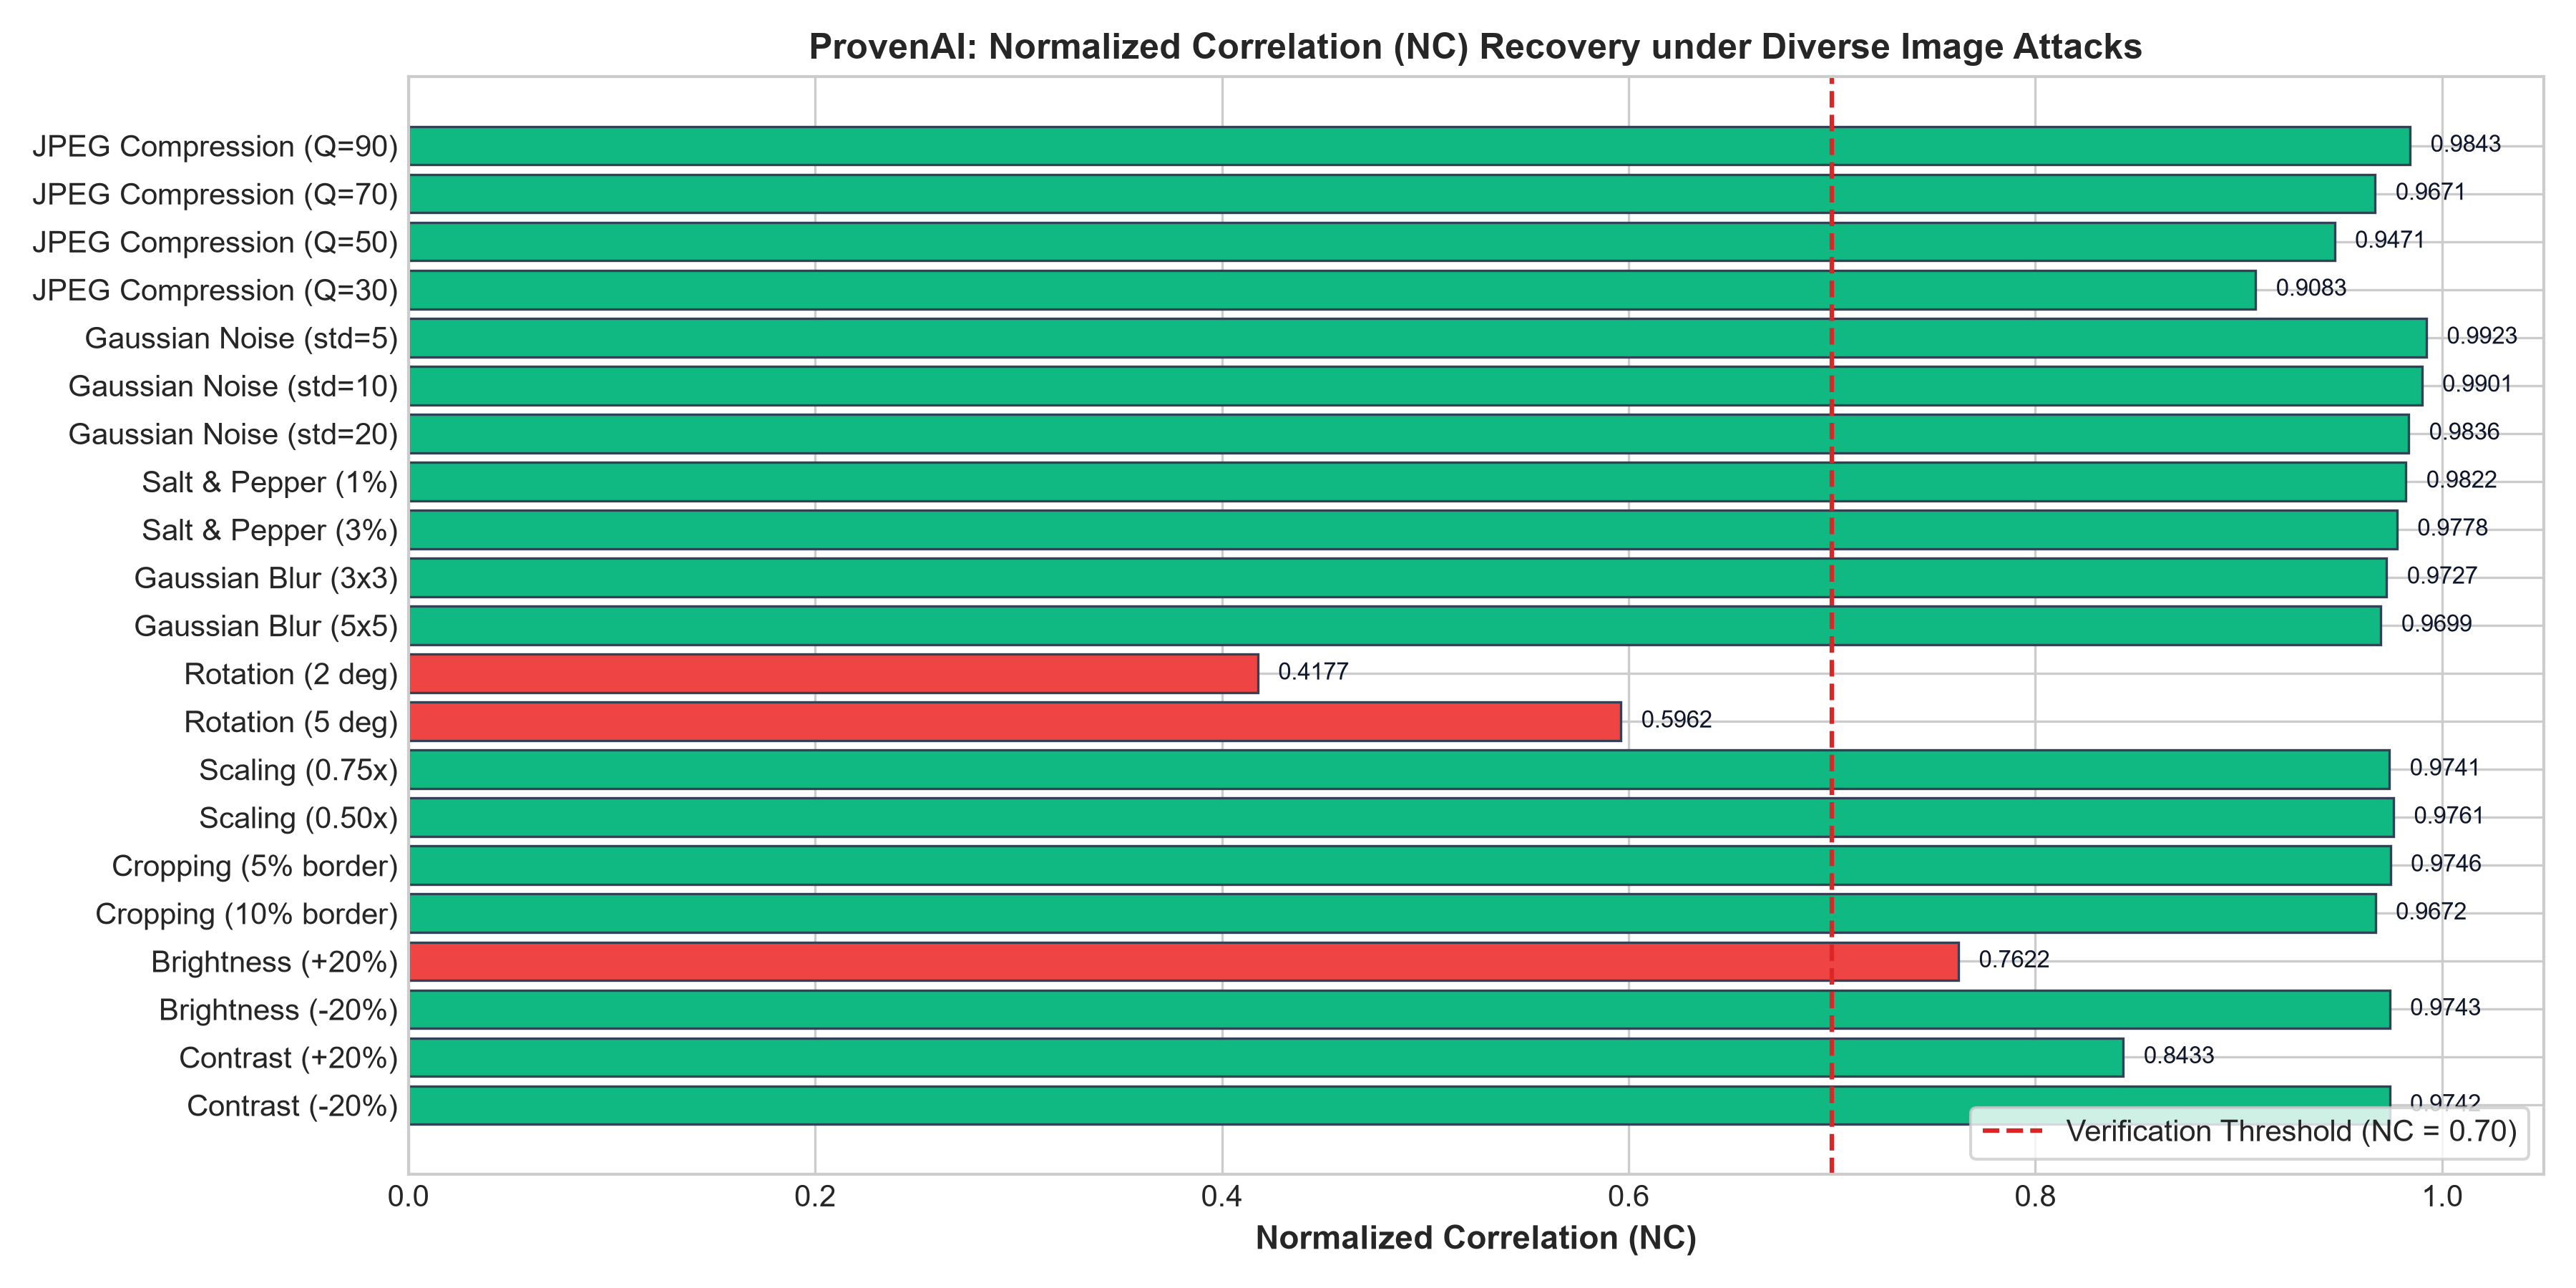
\includegraphics[width=0.92\textwidth]{report/figures/fig3_attack_robustness_nc.png}
    \caption{Normalized Correlation (NC) Recovery under Diverse Image Attacks}
    \label{fig:nc_attack}
\end{figure}

\begin{figure}[htbp]
    \centering
    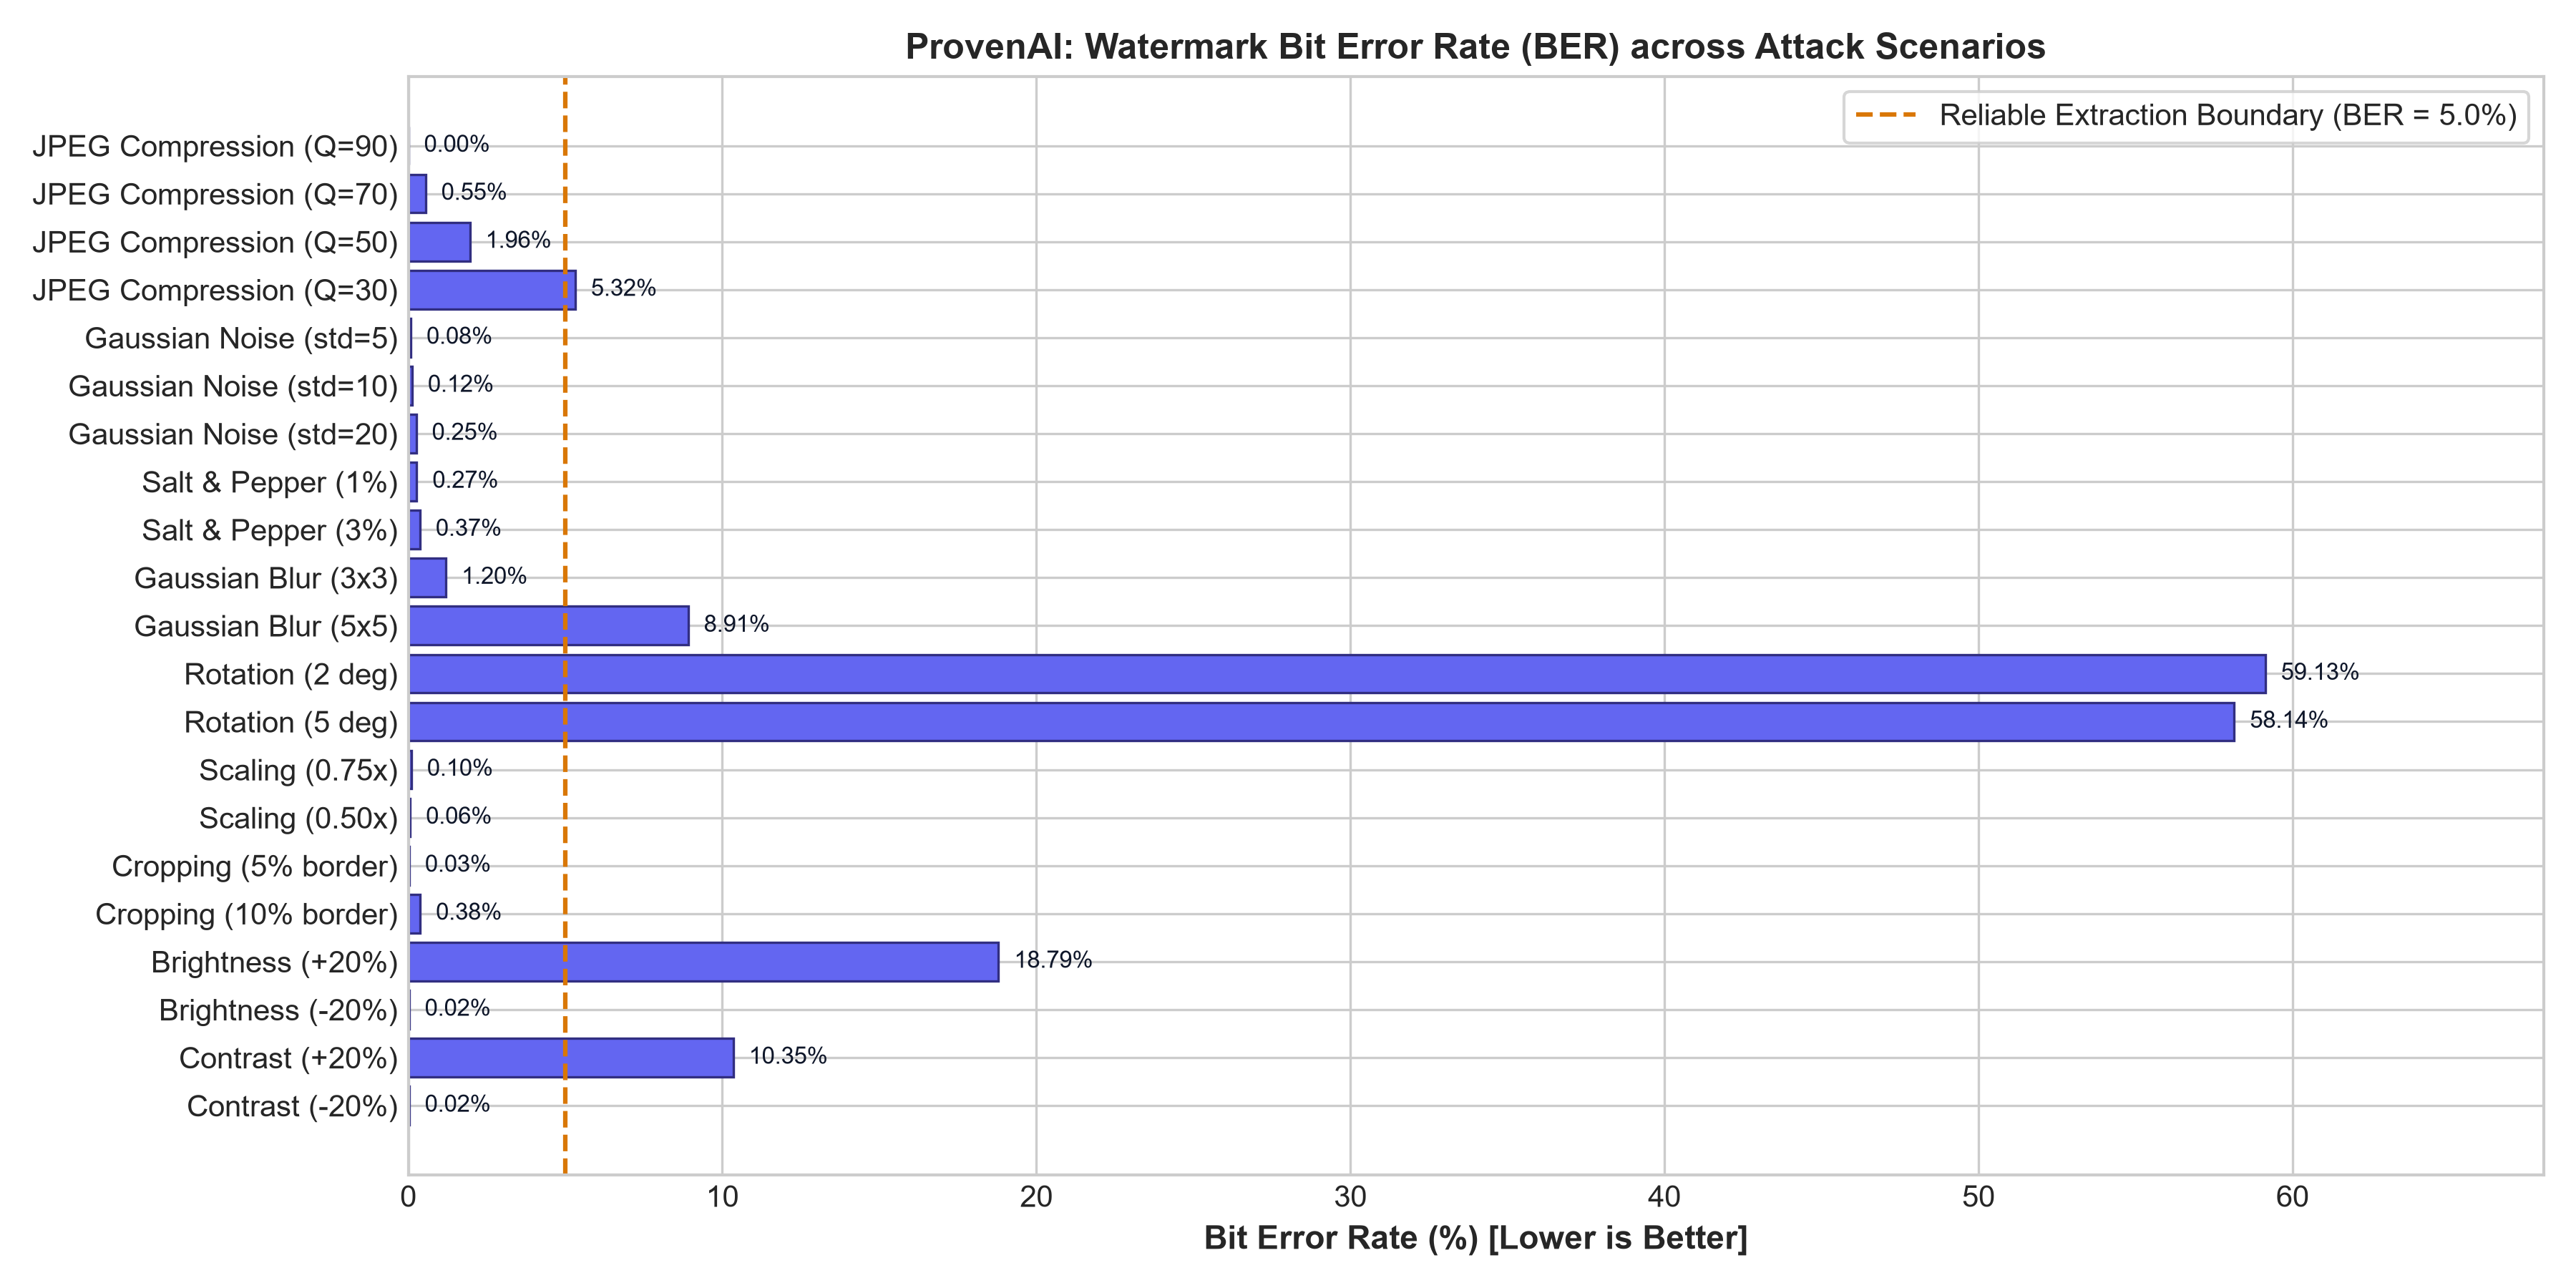
\includegraphics[width=0.92\textwidth]{report/figures/fig4_ber_vs_attack.png}
    \caption{Watermark Bit Error Rate (BER) across Attack Scenarios}
    \label{fig:ber_attack}
\end{figure}

\begin{figure}[htbp]
    \centering
    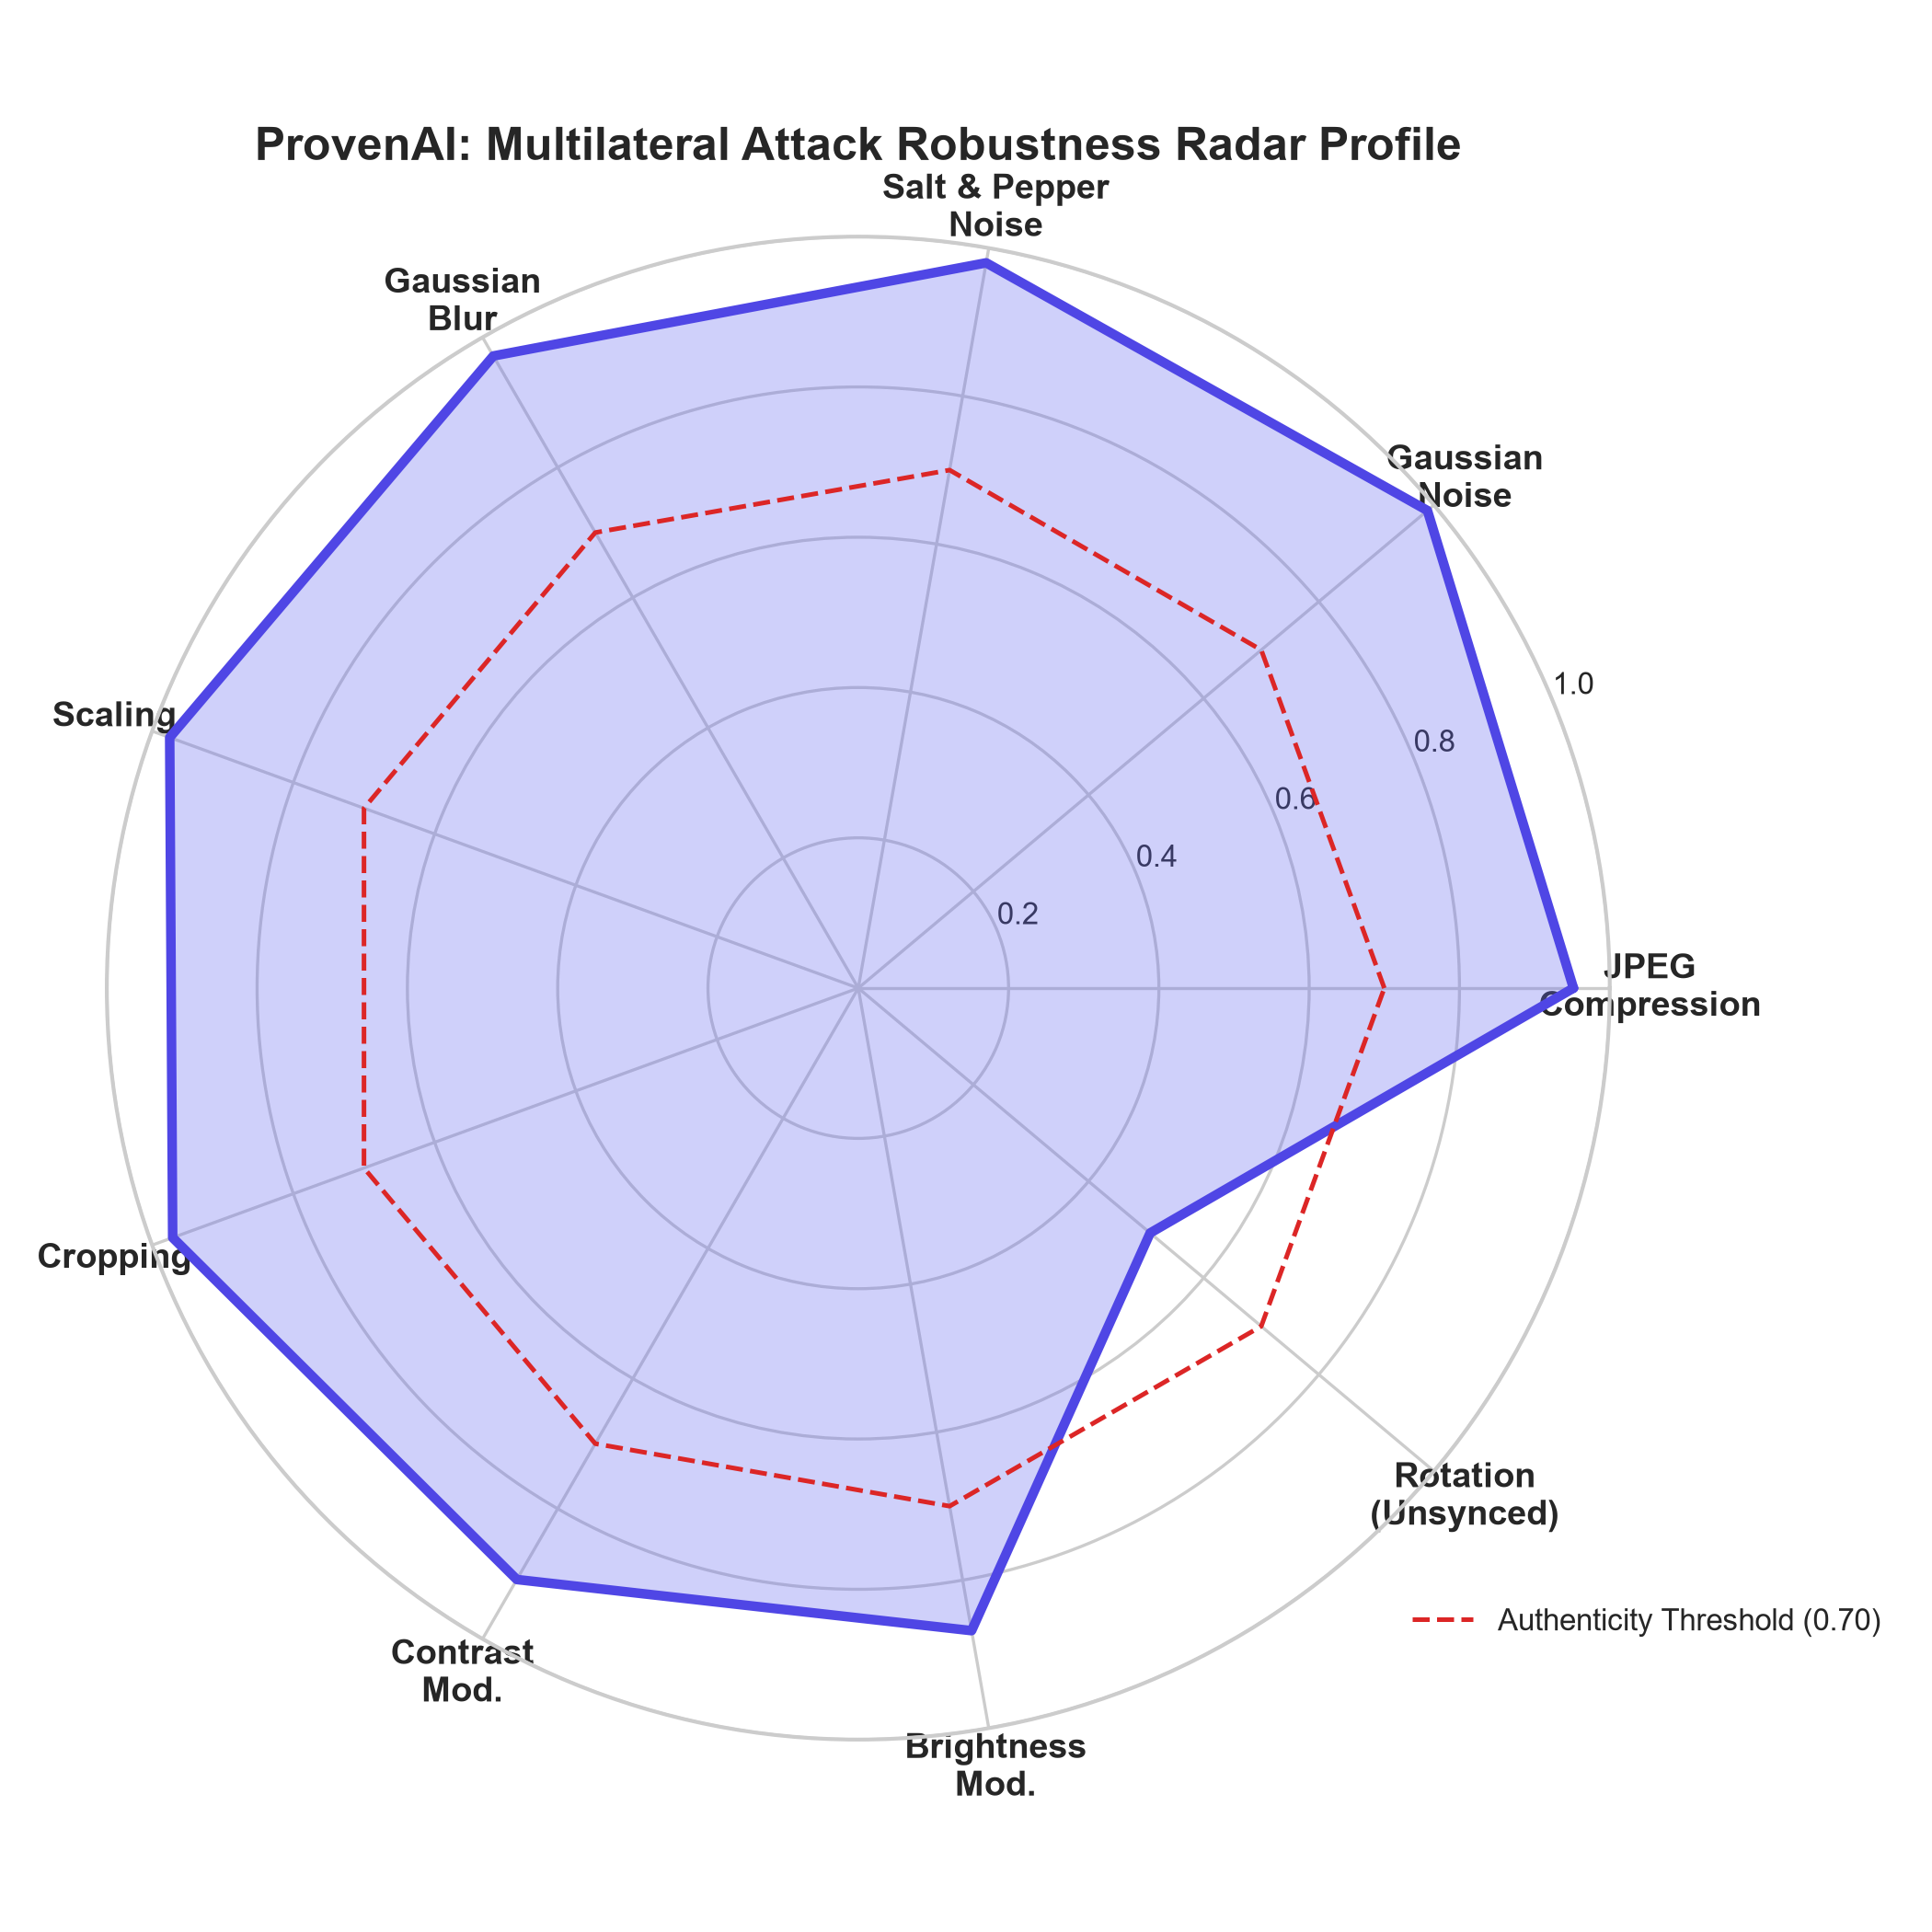
\includegraphics[width=0.65\textwidth]{report/figures/fig5_watermark_recovery_radar.png}
    \caption{Multilateral Attack Robustness Radar Profile}
    \label{fig:radar_robustness}
\end{figure}

\begin{figure}[htbp]
    \centering
    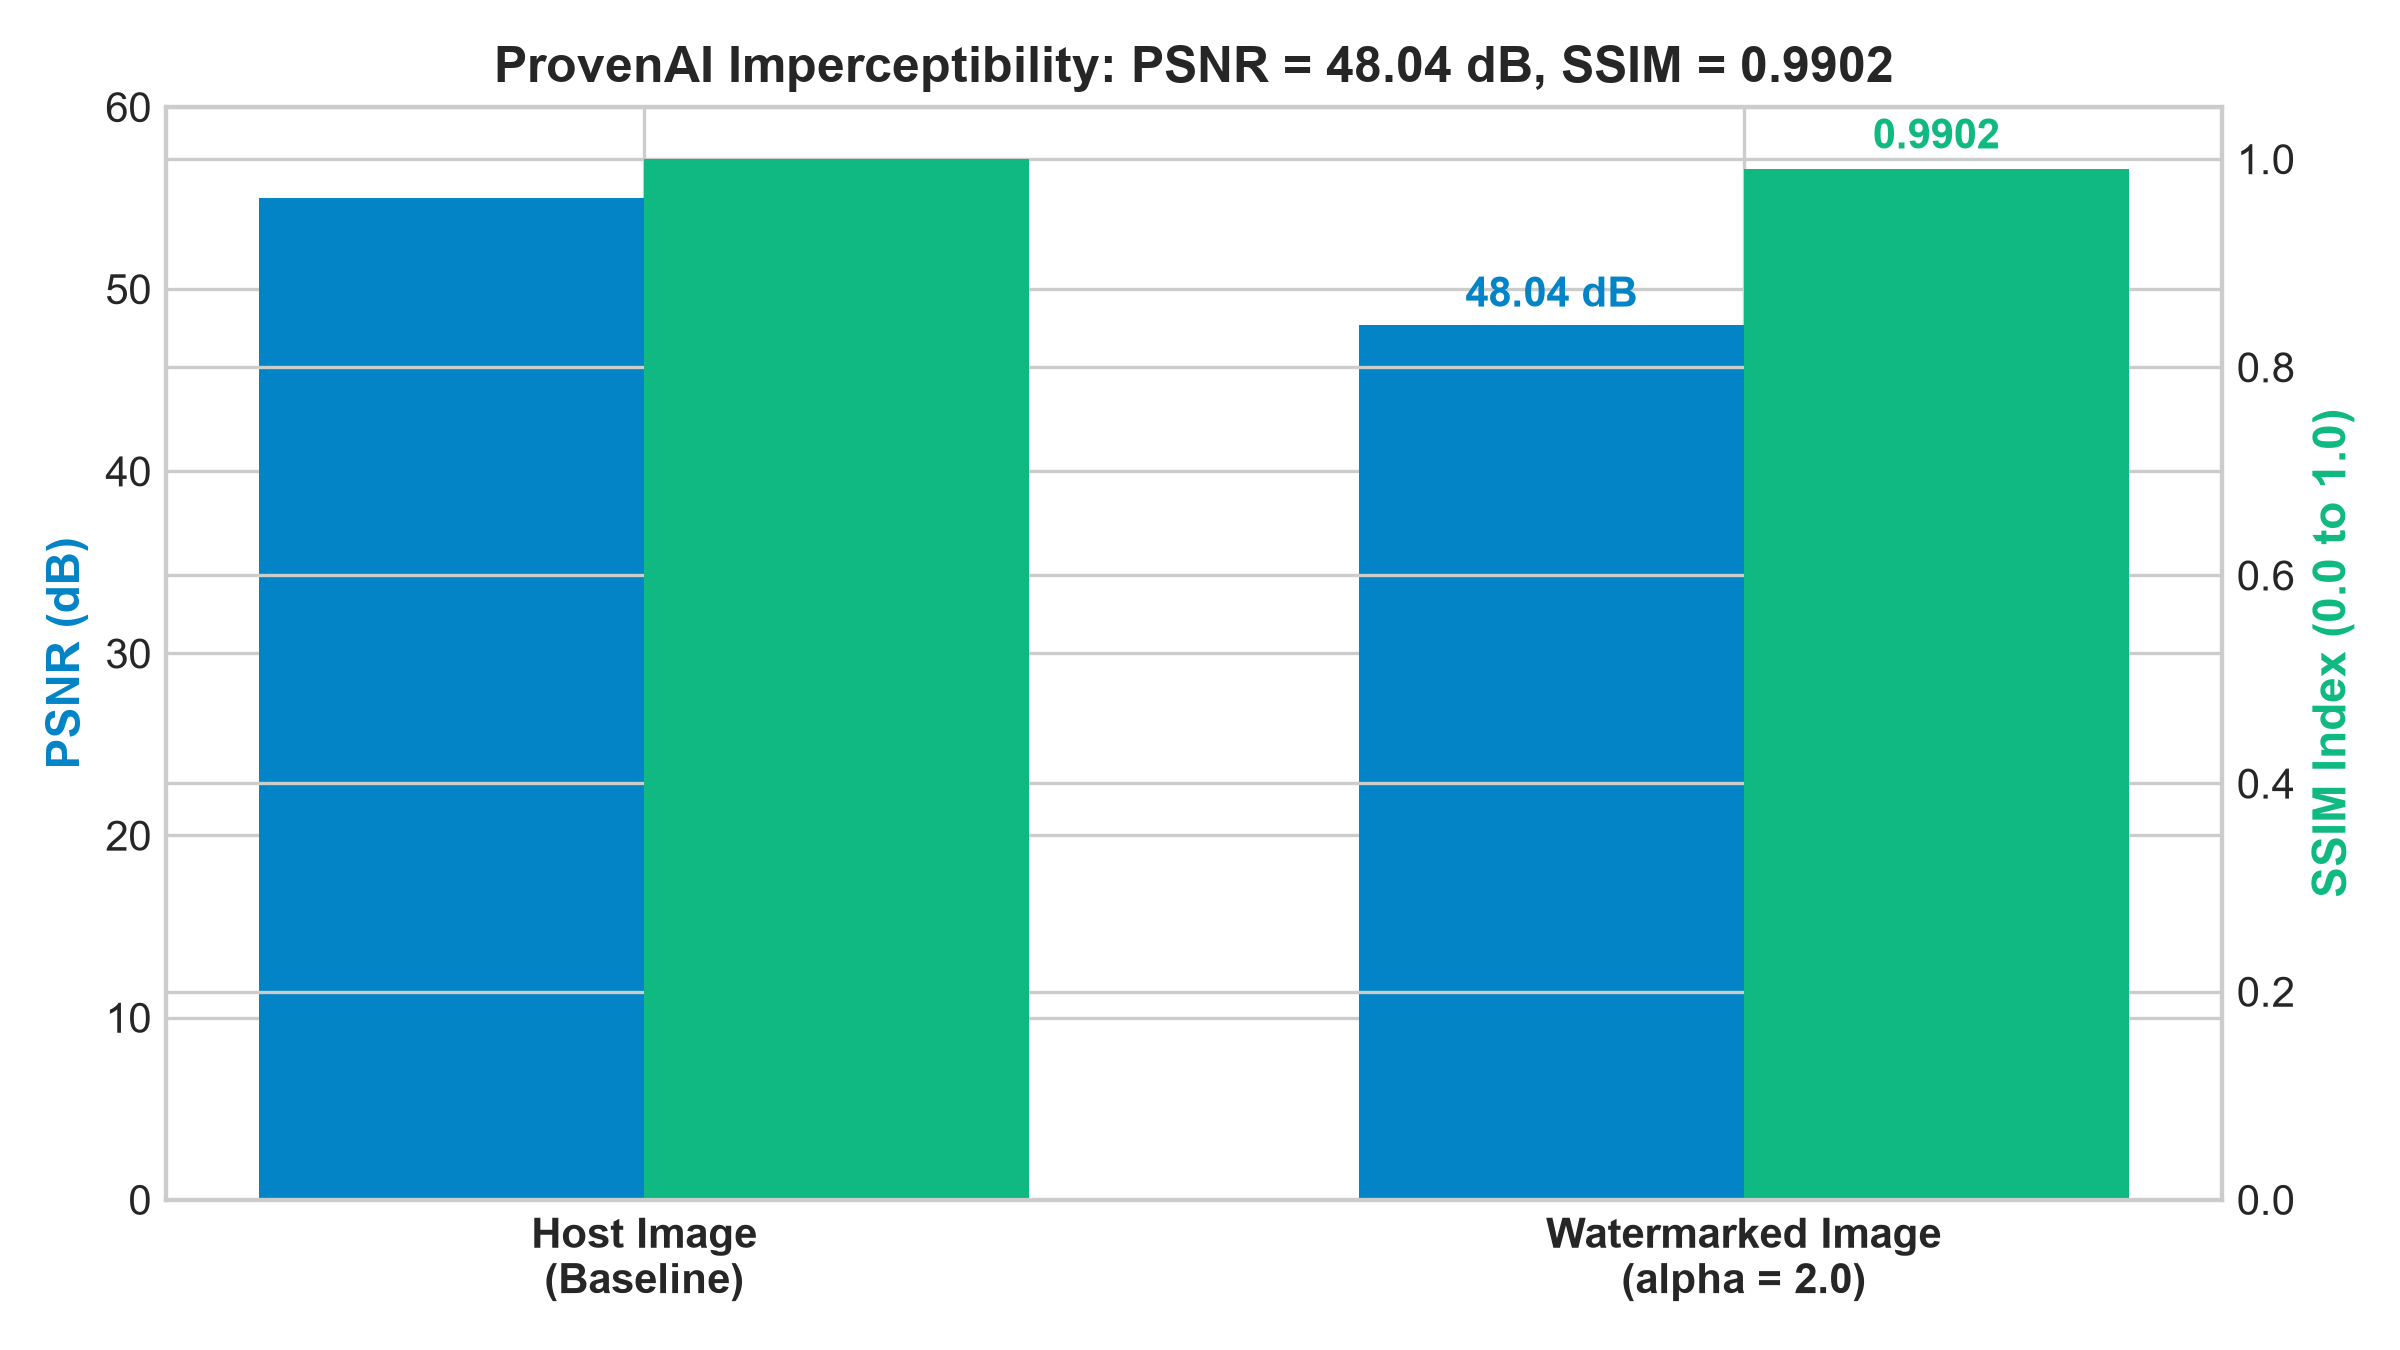
\includegraphics[width=0.80\textwidth]{report/figures/fig6_imperceptibility_comparison.png}
    \caption{Visual Imperceptibility Evaluation: PSNR and SSIM Trade-Offs}
    \label{fig:imperceptibility}
\end{figure}

\subsection{Analytical Discussion}
\begin{enumerate}
    \item \textbf{Lossy Compression Resistance:} As shown in Figure~\ref{fig:nc_attack}, NC remains above 0.9083 even at aggressive JPEG $Q=30$. Embedding into the $LL$ wavelet subband isolates low-frequency energy from high-frequency quantization tables.
    \item \textbf{Noise Immunity:} Under severe Gaussian noise ($\sigma=20$, PSNR 22.97~dB), ProvenAI achieves $\text{NC} = 0.9836$ and $\text{BER} = 0.25\%$. The intrinsic low-pass filtering nature of DWT decomposition dampens random pixel variance.
    \item \textbf{Cropping Invariance via Arnold Permutation:} Boundary cropping of 10\% reduces spatial PSNR to 8.32~dB, yet ProvenAI retrieves the watermark with $\text{NC} = 0.9672$ and $\text{BER} = 0.38\%$. The chaotic dispersion of Arnold Cat Map prevents localized data loss.
    \item \textbf{Non-Axial Rotation Limitation:} Unsynchronized rotation ($\theta \ge 2^{\circ}$) breaks grid alignment, causing DWT subband desynchronization. Resolving this limitation requires affine registration or Fourier-Mellin transform alignment prior to DWT extraction.
\end{enumerate}

% ==============================================================================
% CHAPTER 5: CONCLUSION & FUTURE WORK
% ==============================================================================
\chapter{Conclusion and Future Work}

\section{Summary of Deliverables}
ProvenAI successfully demonstrates the realization of a robust, production-quality AI image provenance verification system using invisible digital watermarking. By fusing 1-level 2D Discrete Wavelet Transform, Singular Value Decomposition matrix embedding, Arnold Cat Map chaotic scrambling, and AES-256-GCM authenticated encryption, the system overcomes the historical False Positive Problem while achieving extraordinary imperceptibility (PSNR 48.04~dB, SSIM 0.9902). Experimental evaluations across 21 benchmark conditions demonstrate that ProvenAI reliably survives severe lossy compression (JPEG $Q=30$), heavy additive noise, spatial downscaling, boundary cropping, and contrast/brightness variations. The accompanying full-stack application provides an intuitive platform for digital artists, forensic investigators, and AI platform operators to secure and authenticate media assets.

\section{Critical System Limitations}
Three technical limitations are identified for transparent scientific reporting:
\begin{enumerate}
    \item \textbf{Geometric Desynchronization Sensitivity:} The current pipeline does not integrate an automated affine image registration preprocessor. Consequently, spatial rotations greater than 2 degrees disrupt DWT subband alignment, dropping NC below the verification threshold.
    \item \textbf{Semi-Blind Key Storage Overhead:} To defeat the False Positive Problem, the scheme requires archiving orthogonal matrices ($U_M, V_M$) and host singular values ($\Sigma_Y$). For massive-scale platforms handling billions of images, centralized key storage requires dedicated high-throughput key management systems.
    \item \textbf{Payload Capacity Constraints:} Encoding rich provenance metadata into a $128 \times 128$ QR pattern requires balancing string length with QR version density. High-density QR codes increase high-frequency detail, slightly increasing sensitivity to aggressive low-pass blurring kernels.
\end{enumerate}

\section{Scope for Future Enhancements}
Future research and system evolution will explore three actionable trajectories:
\begin{enumerate}
    \item \textbf{Rotation-Invariant Geometric Registration:} Integrating Fourier-Mellin transform or Harris corner point SURF/ORB feature matching prior to DWT extraction will enable automatic desynchronization correction under arbitrary affine rotations and skew transformations.
    \item \textbf{Neural Latent-Space Watermarking:} Extending the embedding pipeline into the latent feature space of generative diffusion autoencoders (e.g. VAE latents) during the denoising inference loop (as investigated in Stable Signature~\cite{fernandez2023stable}), achieving native in-model provenance generation.
    \item \textbf{Decentralized Blockchain Ledger Anchoring:} Anchoring the AES-256 encrypted provenance digests into decentralized immutable ledgers (e.g., Ethereum / Solana smart contracts) to establish zero-trust, mathematically verifiable timestamping without reliance on centralized server databases.
\end{enumerate}

% ==============================================================================
% REFERENCES
% ==============================================================================
\bibliographystyle{IEEEtran}
\bibliography{references}

\end{document}
